\section{Interaction Design Process}
Interaction design can be briefly defined as \quotes{designing interactive products to support people in their everyday working lives} \cite{Sharp2011}. To develop a useful product an understanding of what is needed must be established before and during the development process. This brings new challenges and questions, such as if users understand what they are expecting from a specific product, and correctly establishing who the users are beforehand. The interaction design process is a strong user-centred methodology that when correctly carried out will produce an output that reflects the real user's voice and needs. 

Users are the people for whom the system is developed and who will employ it for their goals. Stakeholders are the people that are involved in the development process, influencing the system requirements. For the purposes of this project, the users are both the general public who are concerned with air and its impact on their health status and sensitive users which are at greater risk of suffering health consequences from air pollution. The stakeholders are the secondary agents who have provided an opinion on the capabilities of the system, in this case my project supervisor and other researchers in the field that can give formative feedback.

As described in Figure \ref{fig:interaction_design}, the interaction design process is carried out at four stages: \begin{itemize}
  \item Identify user needs and establishing requirements
  \item Develop alternative designs
  \item Build interactive versions
  \item Evaluate with users
\end{itemize}

\begin{figure}[h]
  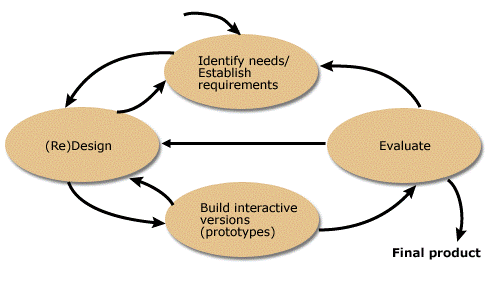
\includegraphics[scale=.8]{images/interatcion-design.png}
  \caption[Interaction design process]{Interaction design process \cite{Sharp2011}.}
  \label{fig:interaction_design}
\end{figure}

Identifying needs and establishing requirements is the first and most crucial activity of the process. Its objective is to learn and understand the user's needs and communicate them to the developer. According to the Chaos report \cite{Group1994}, problems involving requirements account for more than the 30\% of project failures including lack of user input, incomplete requirements and specifications or changes in requirements and specifications. Also, the interdisciplinary nature of requirements elicitation and contradictions between stakeholders add complexity to this part of the process. To make this stage more accurate and disciplined it is useful to combine different techniques and methodologies, such as questionnaires, interviews, introspection and brainstorming \cite{Coulin2005}. The selected methods were questionnaires and interviews. Interviews allowed for casual conversations with a few potential application users, whereas questionnaires allowed for different points of views from many potential users of the application. 

A support tool for developing alternative designs is the prototype, a physical or digital outline of a screen or task supported by the product. This allows for different purposes: first, as support for the creative process, allowing the designer to print the expected interface and how it will support the intended use cases. Second, as a communication tool for the stakeholders, it supports the flow of ideas between the designer and the people involved in the development. Finally, it allows the designer to get measurable feedback of the capabilities of the product. Prototypes were designed and evaluated in different iterations across the project.